\documentclass[12pt, letterpaper]{article}
\usepackage{graphicx}
\graphicspath{{images/}}

\title{CCE5225 - Assignment 1 \\
\large MiniBooNE particle identification \\ signal/background classification}
\author{Sultan Dayani}
\date{December 2022}
\begin{document}
\maketitle
\pagebreak

\textgreater{Comment on whether the performance changes significantly amongst different hyperparameter values for each model.}
\textgreater{Report the time required for training, the set of hyperparameters which were tested, and the final per-class accuracies achieved on the unseen test set (in the form of a confusion matrix).}
\textgreater{Comment on the performance of each model, and provide an explanation as to why you believe the highest performing model gave the best results.}

# 1 Hidden Layer
Params: 'hidden_layer_sizes': [(10,), (20,), (30,), (40,), (50,)]
\begin{tabular}{|c c c|}
\hline
HL Size & Mean Fit Time & Mean Score \\ [0.5ex] 
\hline
(10,) & 99.88s & 0.927113 \\
\hline
(20,) & 100.26s & 0.931188 \\
\hline
(30,) & 74.61s & 0.933052 \\
\hline
(40,) & 376.35s & 0.935090 \\
\hline
(50,) & 163.39s & 0.933744 \\ 
\hline
\end{tabular}
Vanilla Neural Network best hyperparameters: {'hidden_layer_sizes': (40,), 'max_iter': 500, 'random_state': 42}
Vanilla Neural Network best cross-validation accuracy: 0.935090
The best performing model was the neural network with 40 neurons.
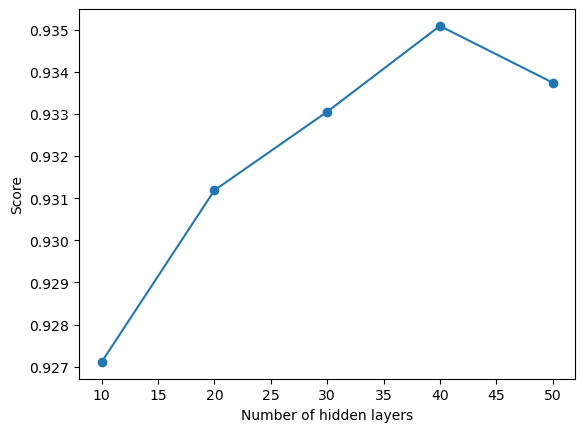
\includegraphics[width=0.6\textwidth]{1hiddenlayer_scores.png}

# Increasing the number of hidden layers
Choosing 30 for the size of neurons per hidden layer as it is the best performing size from the previous models.
Params: 'hidden_layer_sizes': [(40,), (40,40), (40,40,40), (40,40,40,40)],
HiddenLayerSize: (40,) | 75.29s | test-score: 0.935311
HiddenLayerSize: (40, 40) | 86.75s | test-score: 0.936723
HiddenLayerSize: (40, 40, 40) | 163.92s | test-score: 0.934984
HiddenLayerSize: (40, 40, 40, 40) | 249.26s | test-score: 0.932158



#SVM
hyperparameters: 'C': [0.1, 1, 10],
C: 0.1 | 331.12s | test-score: 0.877185
C: 1 | 160.40s | test-score: 0.891601
C: 10 | 148.25s | test-score: 0.906661
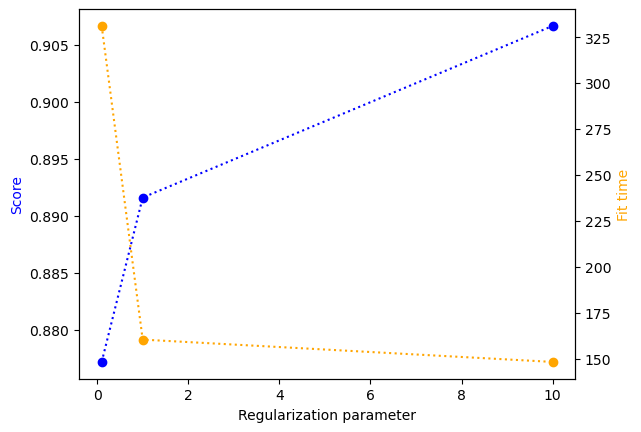
\includegraphics[width=0.6\textwidth]{svm_c_compiled.png}



\end{document}